\documentclass[a4paper,12pt]{foi}

\renewcommand{\brojAutora}{1} % Broj autora rada (max. 6)
\renewcommand{\naslov}{Naslov rada} % Naslov rada
\renewcommand{\mentor}{Doc. dr. sc. Markus Schatten} % Ime i prezime mentora
\renewcommand{\autorA}{Ime Prezime} % Ime i prezime prvog autora
\renewcommand{\brIndeksaA}{43201} % Broj indeksa prvog autora
\renewcommand{\vrstaRada}{Diplomski rad} % Vrsta rada: Seminarski rad, Pristupni rad, Projekt ...

\begin{document}

\maketitle

\tableofcontents

\thispagestyle{empty}

\setcounter{page}{0}

\onehalfspacing

\chapter{Uvod}

Ovo je \LaTeXe\ predlo\v{z}ak za pisanje seminarskih, pristupnih, projektnih i drugih radova na Fakultetu organizacije i informatike.

\chapter{Slike}

Za prikaz slika mo\v{z}e se koristiti sljede\'{c}a sintaksa (\ref{slika-1}).

\begin{figure}[h]
\centering 
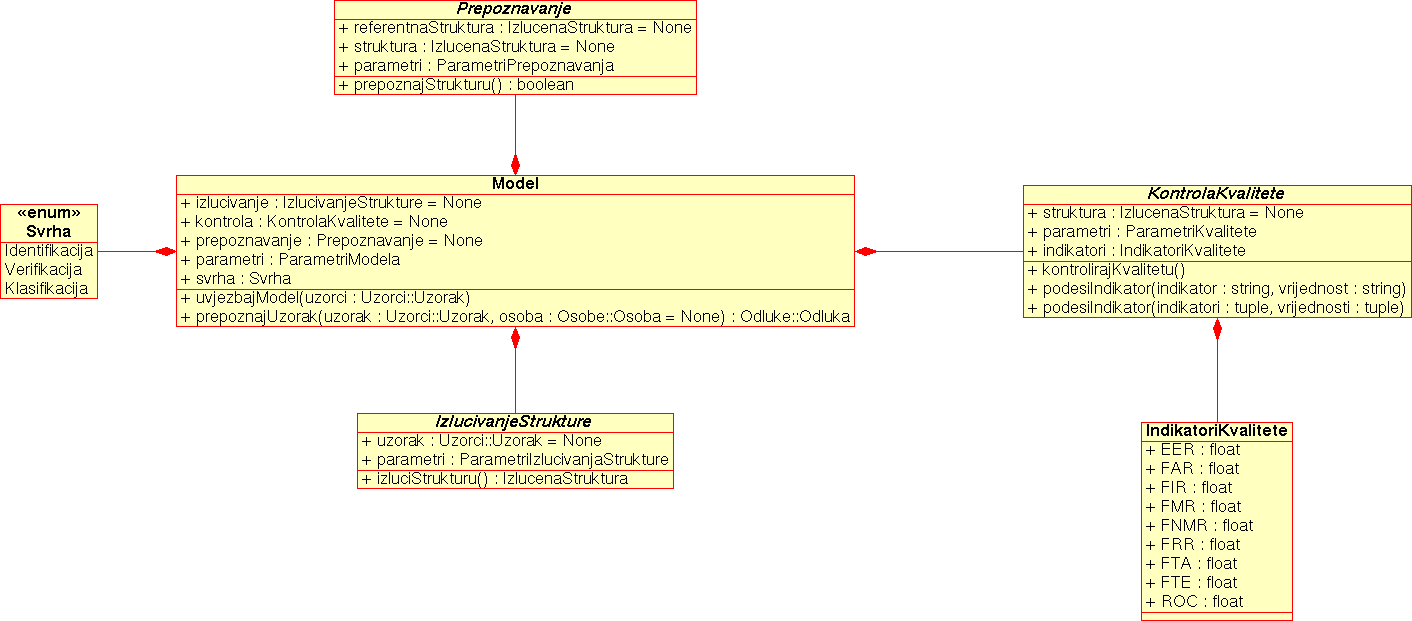
\includegraphics[width=0.95\textwidth]{model.png}
\caption{UML model za biometrijske sustave \citep{Schatten2008}}
\label{slika-1}
\end{figure}

Pri \v{c}emu su podr\v{z}ani formati png, pdf, jpg i jpeg. Drugi su formati mogu\'{c}i uz dodavanje odgovaraju\'{c}ih opcija.

\chapter{Tablice}

Primjer tablice (vidi tablicu \ref{tablica-1}) u kojoj su prikazani neki faktori.


\begin{table}[h]
\caption{Tablica nekih faktora}
\begin{center}
\begin{tabular}{||c|r|r||}
\hline
\textbf{Faktor}&\textbf{Opis}&\textbf{Vrijednost} \\
\hline
Faktor 1&opis 1&121.23 \\
Faktor 2&opis 2&65.56 \\
Faktor 3&opis 3&27.09 \\
Faktor 4&opis 4&18.08 \\
\hline
\end{tabular}
\end{center}
\label{tablica-1}
\end{table}

\chapter{Formule}

\LaTeXe\ je poznat po svojoj podr\v{s}ci za formule (izraz \ref{formula}):

\begin{equation}
 \label{formula}
 \displaystyle\sum_{i \in \{ 0, 1, 2, 3, \cdots, n\}}{\frac{w_i \times \sqrt{4 - \epsilon_i}}{\frac{\varphi}{\Upsilon}}}
\end{equation} 

Da biste se referencirali na neku formulu u tekstu potrebno je formulu dati naziv (naredba \texttt{label}) te na mjestu citiranja koristiti naredbu \texttt{ref} s navedenim nazivom. Ako ne želite da se formule numeriraju koristite naredbu \texttt{\textbackslash begin\{equation*\}}.

\chapter{Hiperveze}

U predlo\v{s}ku su omogu\'{c}ene i hiperveze oblika \url{http://cb.foi.hr}. Koristi se naredba \texttt{url} uz \texttt{hyperref} modul koji omogućava automatsko povezivanje pri kliku.

\chapter{Programski k\^{o}d}

Primjer programskog k\^{o}da prikazan je u nastavku:

\definecolor{lbcolor}{rgb}{0.9,0.9,0.9}
\lstset{commentstyle=\textit,language=python}
\lstset{backgroundcolor=\color{lbcolor},rulecolor=}
\begin{lstlisting}[frame=tb]{}
# map.py
# We can use append here
def map( fun, list ):
    nlist = []
    for item in list:
        nlist.append( fun( item ) )
    return nlist
# But here we have to use concatenation, or the + operator for lists.
def rmap ( fun, list ):
    if list == []:
        return []
    else:
        return [fun( list[0] )] + rmap( fun, list[1:] )

# Make a sample test function
def increment(x):
    return x+1

# Test them out!
map( increment, [1,2,3,4,5] )
# should return [2,3,4,5,6]
map( increment, [1,2,3,4,5] ) == rmap( increment, [1,2,3,4,5] )
# There outputs should be the same!

\end{lstlisting}

Dobro je proučiti modul \texttt{lstlisting} jer ima mnogo interesantnih opcija za formatiranje k\^{o}da poput dodavanja brojeva linija, različitih boja za različite ključne riječi i sl.

\chapter{Citiranje literature}

Za potrebe citiranja kori\v{s}tene literature koristi se datoteka foi.bib (BiBteX format) u kojoj valja postaviti odgovaraju\'{c}e reference. U postoje\'{c}oj datoteci postoje primjeri za knjige \citep{Baral2004, Jennex2007, JohsansenSwigart2000, PogacnikBloom1998}, \v{c}lanke u \v{c}asopisima \citep{BacaEtAl2007, Jurin2006}, \v{c}lanke u uredni\v{c}kim knjigama \citep{Garzarelli2004, Luhmann2003}, \v{c}lanke u zbornicima konferencija \citep{AbeleBischoff2001, BacaEtAl2006}, zatim doktorske disertacije \citep{Bahr2009}, magistarske radove \citep{Schatten2008}, priru\v{c}nike (manuale) \citep{HAZU2004}, tehni\v{c}ke izvje\v{s}taje \citep{BlonkEtAll1998}, kao i Internet reference \citep{Berger2006, Pilgrim2006}. Citiranjem pojedinih referenci u tekstu (naredba \texttt{citep}) \LaTeXe\ automatski generira bibliografiju na kraju dokumenta.

\addcontentsline{toc}{chapter}{Bibliografija}
\bibliography{foi.bib}
\end{document}
